\documentclass[t,usepdftitle=false]{beamer}
\usepackage[utf8]{inputenc}
\usetheme{Warsaw}
\usepackage{xcolor}

\usepackage{etex}
\usepackage{pictex}
\usepackage{tikz}
\usetikzlibrary{shapes,arrows}
\usepackage{pgfplots}

\usepackage{graphicx}

\usepackage{amsmath}
\usepackage{amscd}
\usepackage{pstricks, pst-node}

\usepackage{times}

\usepackage{ulem}

\usepackage{amsmath, amsthm}
\usepackage{listings}

% \setbeamercovered{transparent}
%\usecolortheme{crane}
\title[IFT3245]{IFT 3245\\Simulation et modèles}
\author[Fabian Bastin]{Fabian Bastin\\DIRO\\Université de Montréal}
\date{Automne 2016}

\def\be{\boldsymbol{e}}
\def\bh{\boldsymbol{h}}
\def\bu{\boldsymbol{u}}
\def\bv{\boldsymbol{v}}
\def\bx{\boldsymbol{x}}
\def\bA{\boldsymbol{A}}
\def\bC{\boldsymbol{C}}
\def\bP{\boldsymbol{P}}
\def\bU{\boldsymbol{U}}
\def\bX{\boldsymbol{X}}
\def\bY{\boldsymbol{Y}}

\def\bone{\boldsymbol{1}}

\def\q{\quad}

\def\bbeta{\boldsymbol{\beta}}
\def\bmu{\boldsymbol{\mu}}
\def\bnu{\boldsymbol{\nu}}
\def\bSigma{\boldsymbol{\Sigma}}
\def\bzero{\boldsymbol{0}}

\def\eqas{\overset{\mbox{p.s.}}{=}}

\def\cA{\mathcal{A}}
\def\cH{\mathcal{H}}
\def\cJ{\mathcal{J}}
\def\cN{\mathcal{N}}
\def\cS{\mathcal{S}}

\def\rit{\mathcal{R}}
\def\NN{\mathcal{N}}
\def\RR{\mathcal{R}}
\def\ZZ{\mathcal{Z}}

\def\eps {$< 10^{-15}$}
\def\epsm {$> 1-10^{-15}$}

\def\MSE{\mbox{MSE}}
\def\RE{\mbox{RE}}
\def\eff{\mbox{Eff}}
\def\Var{\mbox{Var}}
\def\Cov{\mbox{Cov}}
\def\var{\mbox{var}}

\def\iid{i.i.d.}
\def\toas{\mbox{ to as }}
\def\To{\overset{D}{\to}}

\newtheorem{assumption}{Hypothèse}
\newtheorem{thm}{Theorème}
\newtheorem{defn}{Définition}
\newtheorem{coro}{Corollaire}
\newtheorem{prop}{Proposition}
\newtheorem{exe}{Exemple}

\begin{document}
\frame{\titlepage}

\begin{frame}
\frametitle{Variables antithétiques (AV)}

Semblable \`a l'idée des VAC, sauf que l'on veut maintenant estimer
\emph{une seule espérance} par un moyenne de plusieurs estimateurs
\emph{négativement corrélés}.

\mbox{}

Supposons que l'on a ${k}$ estimateurs sans biais de ${\mu}$,
$({X^{(1)}},\dots, {X^{(k)}})$, avec 
$\Var[X^{(1)}] = \cdots = \Var[X^{(k)}]$.

\mbox{}

La moyenne
\[
  {X_{\rm a}} = \frac{1}{k}\sum_{\ell=1}^k X^{(\ell)}
\]
est un estimateur \emph{sans biais} de $\mu$, avec variance 
\[
 {\Var[X_{\rm a}]} = 
  \frac{1}{k^2} \sum_{j=1}^k \sum_{\ell=1}^k \Cov[X^{(j)}, X^{(\ell)}] 
  = \frac{\Var[X_{(1)}]}{k} 
     + \frac{2}{k^2}\sum_{j<\ell} \Cov[X^{(j)}, X^{(\ell)}].
\]

\end{frame}

\begin{frame}
\frametitle{Variables antithétiques}

Si les $X^{(\ell)}$ sont indépendants, les covariances sont nulles.

\mbox{}

La variance est réduite ssi $\Var[X_{\rm a}] < \Var[X_{(1)}]/{k}$, \\
ssi la somme des covariances est négative.

\mbox{}

Pour un total de ${n} = mk$ répétitions, on définit
\[
  {\bar X_{\rm a,n}} 
   = {1\over m} \sum_{i=1}^{m} X_{\rm a,i}
   = {1\over n} \sum_{i=1}^{m} \sum_{\ell=1}^k X_i^{(\ell)},
\]
o\`u ${X_{\rm a,1}}, \dots, {X_{\rm a,m}}$
sont des copies \iid\ de $X_{\rm a}$.

\mbox{}

Estimateur sans biais de $\Var[X_{\rm a}]$; variance empirique:
\[
  {S_{\rm a,m}^2} 
  = {1\over m-1} \sum_{i=1}^{m} 
    \left(X_{\rm a,i} - \bar X_{\rm a,n}\right)^2.
\]

\end{frame}

\begin{frame}
\frametitle{Méthode AV générale}

Soit ${\mu} = E[X]$, o\`u ${X} = f(\bU)$ et 
$\bU = ({U_1},{U_2},\dots)$ une suite \iid{} $U(0,1)$.
Pour ${\ell}=1,\dots,k$, soit ${X^{(\ell)}} = f(\bU^{(\ell)})$ 
o\`u ${\bU^{(\ell)}}$ est une suite \iid{} $U(0,1)$.

\mbox{}

Le but de l'approche de variables antithétiques généralisées est
d'induire une dépendance entre les $\bU_\ell$ de manière \`a rendre
$\sum_{j<\ell} \Cov[X^{(j)}, X^{(\ell)}] < 0$.

\end{frame}

\begin{frame}
\frametitle{Paires antithétiques}

On a ${k}=2$,\\
\q ${\bU^{(1)}} = \bU = (U_1,U_2,\dots)$, \\
\q ${\bU^{(2)}} = \bone -\bU = (1-U_1, 1-U_2, \dots)$, 
la \emph{suite antithétique}.

\mbox{}

Posons ${X_{\rm a}} = [X^{(1)} + X^{(2)}]/2$,
\begin{eqnarray*}
 {\Var[X_{\rm a}]}
    &=& {(\Var[X^{(1)}] + \Var[X^{(2)}] + 2 \, \Cov[X^{(1)}, X^{(2)}]) / 4} \\
    &=& {(\Var[X^{(1)}] + \Cov[X^{(1)}, X^{(2)}]) / 2},
\end{eqnarray*}
et $\Var[X_{\rm a}] < \Var[X]/2$ \ ssi \ $\Cov[X^{(1)}, X^{(2)}] < 0$.

\mbox{}

\emph{Intuition}:
Les événements désastreux pour $X^{(1)}$ seront compensés par
des événements antithétiques chanceux pour $X^{(2)}$, et vice-versa.

%{\bf Exemple.}  \emph{Réseau d'activités stochastique.}\\
%On veut estimer $\mu = P[T > x]$, o\`u ${T}$ est la longueur du
%plus long chemin et ${x}$ une constante.  

%On génère $V_j = F_j^{-1}(U_j)$ pour $X^{(1)}$ et
%$V_j = F_j^{-1}(1-U_j)$ pour $X^{(2)}$.

\end{frame}

\begin{frame}
\frametitle{Mise en oeuvre}
	
	Meilleur cas possible: pour une fonction lin\'eaire la variance est 
	r\'eduite \`a z\'ero.\\
	Pire cas: si $X^{(1)}$ et $X^{(2)}$ sont parfaitement corr\'el\'ees,
	la variance est doubl\'ee (e.g., $f(\bU) = |U_1-1/2|$).
	
	\mbox{}	
	
	Pour \emph{minimiser la covariance}, il faudrait g\'en\'erer
	directement ${X^{(1)}} = F^{-1}(U)$ et ${X^{(2)}} = F^{-1}(1-U)$, 
	o\`u $U \sim U(0,1)$ et $F$ est la fonction de r\'epartition de $X$.
		\\
		Pas pratique.
	
	\mbox{}
	
	Comme pour les VAC, on appliquera l'inversion pour maximiser 
	la covariance \`a un plus bas niveau.
	
	
\end{frame}
%%%%%%%%%%%%%%%%%%%%%%%%%%%%%%

\begin{frame}
\frametitle{Combinaison VAC-AV}

Supposons que l'on veut comparer deux systèmes en utilisant des VAC, 
et aussi des paires de répétitions antithétiques.

Si ces deux méthodes fonctionnent bien séparément, 
fera-t-on nécessairement mieux en les combinant~? \emph{Non}.

Soit ${X^{(1)}_{k}} = f_k(\bU)$ et ${X^{(2)}_{k}} = f_k(\bone-\bU))$, % la paire antithétique,
$k = 1, 2$.  On a 
\begin{small}
\begin{eqnarray*}
 && \Var\left[\frac{ X^{(1)}_{2} + X^{(2)}_{2}}{2} 
            - \frac{ X^{(1)}_{1} + X^{(2)}_{1}}{2}\right] \\ 
 &=&  {\Var[X^{(1)}_{1}] + \Var[X^{(2)}_{1}]
     + \Var[X^{(1)}_{2}] + \Var[X^{(2)}_{2}] \over 4}\\
 && +~{\Cov[X^{(1)}_{1},X^{(2)}_{1}] + \Cov[X^{(1)}_{2},X^{(2)}_{2}] \over 2}
    -~{\Cov[X^{(1)}_{1},X^{(1)}_{2}] + \Cov[X^{(2)}_{1},X^{(2)}_{2}] \over 2}\\
 && -~{\Cov[X^{(2)}_{1},X^{(1)}_{2}] + \Cov[X^{(1)}_{1},X^{(2)}_{2}] \over 2}.\\
 &=&  \Var[X^{(1)}_{1}] 
    + \underbrace{\Cov[X^{(1)}_{1},X^{(2)}_{1}]}_{{\le 0}}
    - \underbrace{\Cov[X^{(1)}_{1},X^{(1)}_{2}]}_{{\ge 0}} 
    - \underbrace{\Cov[X^{(2)}_{1},X^{(1)}_{2}]}_{{?}}.
\end{eqnarray*}
\end{small}

\end{frame}

\begin{frame}
\frametitle{Cas multidimensionnel}

Un \'echantillonnage est \emph{AV-concordant} si $U_{2,j} = 1-U_{1,j}$ 
pour certaines coordonn\'ees $j$ telles que $f$ est monotone par rapport
\`a $U_j$, tandis que $U_{2,j}$ est ind\'ependant de $U_{1,j}$ pour les autres
coordonn\'ees. 

\mbox{}

\begin{thm}
Pour un \'echantillonnage AV-concordant, on a $\Cov[X^{(1)}, X^{(2)}] \le 0$.
\end{thm}


%\emph{Preuve:} en prenant $f_1 = f_2 = f$, VAC-discordant est \'equivalent
%\`a AV-concordant, et le r\'esultat d\'ecoule du th\'eor\`eme sur les VAC.

\end{frame}

\begin{frame}[fragile]
	\frametitle{Un r\'eseau d'activit\'es stochastique.}
	
	Graphe acyclique $(\cN, \cA)$, de \emph{noeuds} ${\cN}$ et 
	\emph{arcs} ${\cA}$ (les activit\'es).\\
	Le graphe donne les relations de pr\'ec\'edence entre les activit\'es.
	Chaque activit\'e $k \in\cA$ a une dur\'ee al\'eatoire ${V_k}$ de
	fonction de r\'epartition $F_k$.\\
	Si $V_k$ est la longueur de l'arc $k$, la dur\'ee minimale du projet
	est la longueur ${T}$ du plus long chemin dans le r\'eseau.\\
	On peut vouloir estimer $P[T > x]$ pour un certain $x$, par exemple.
	
	\begin{center}
		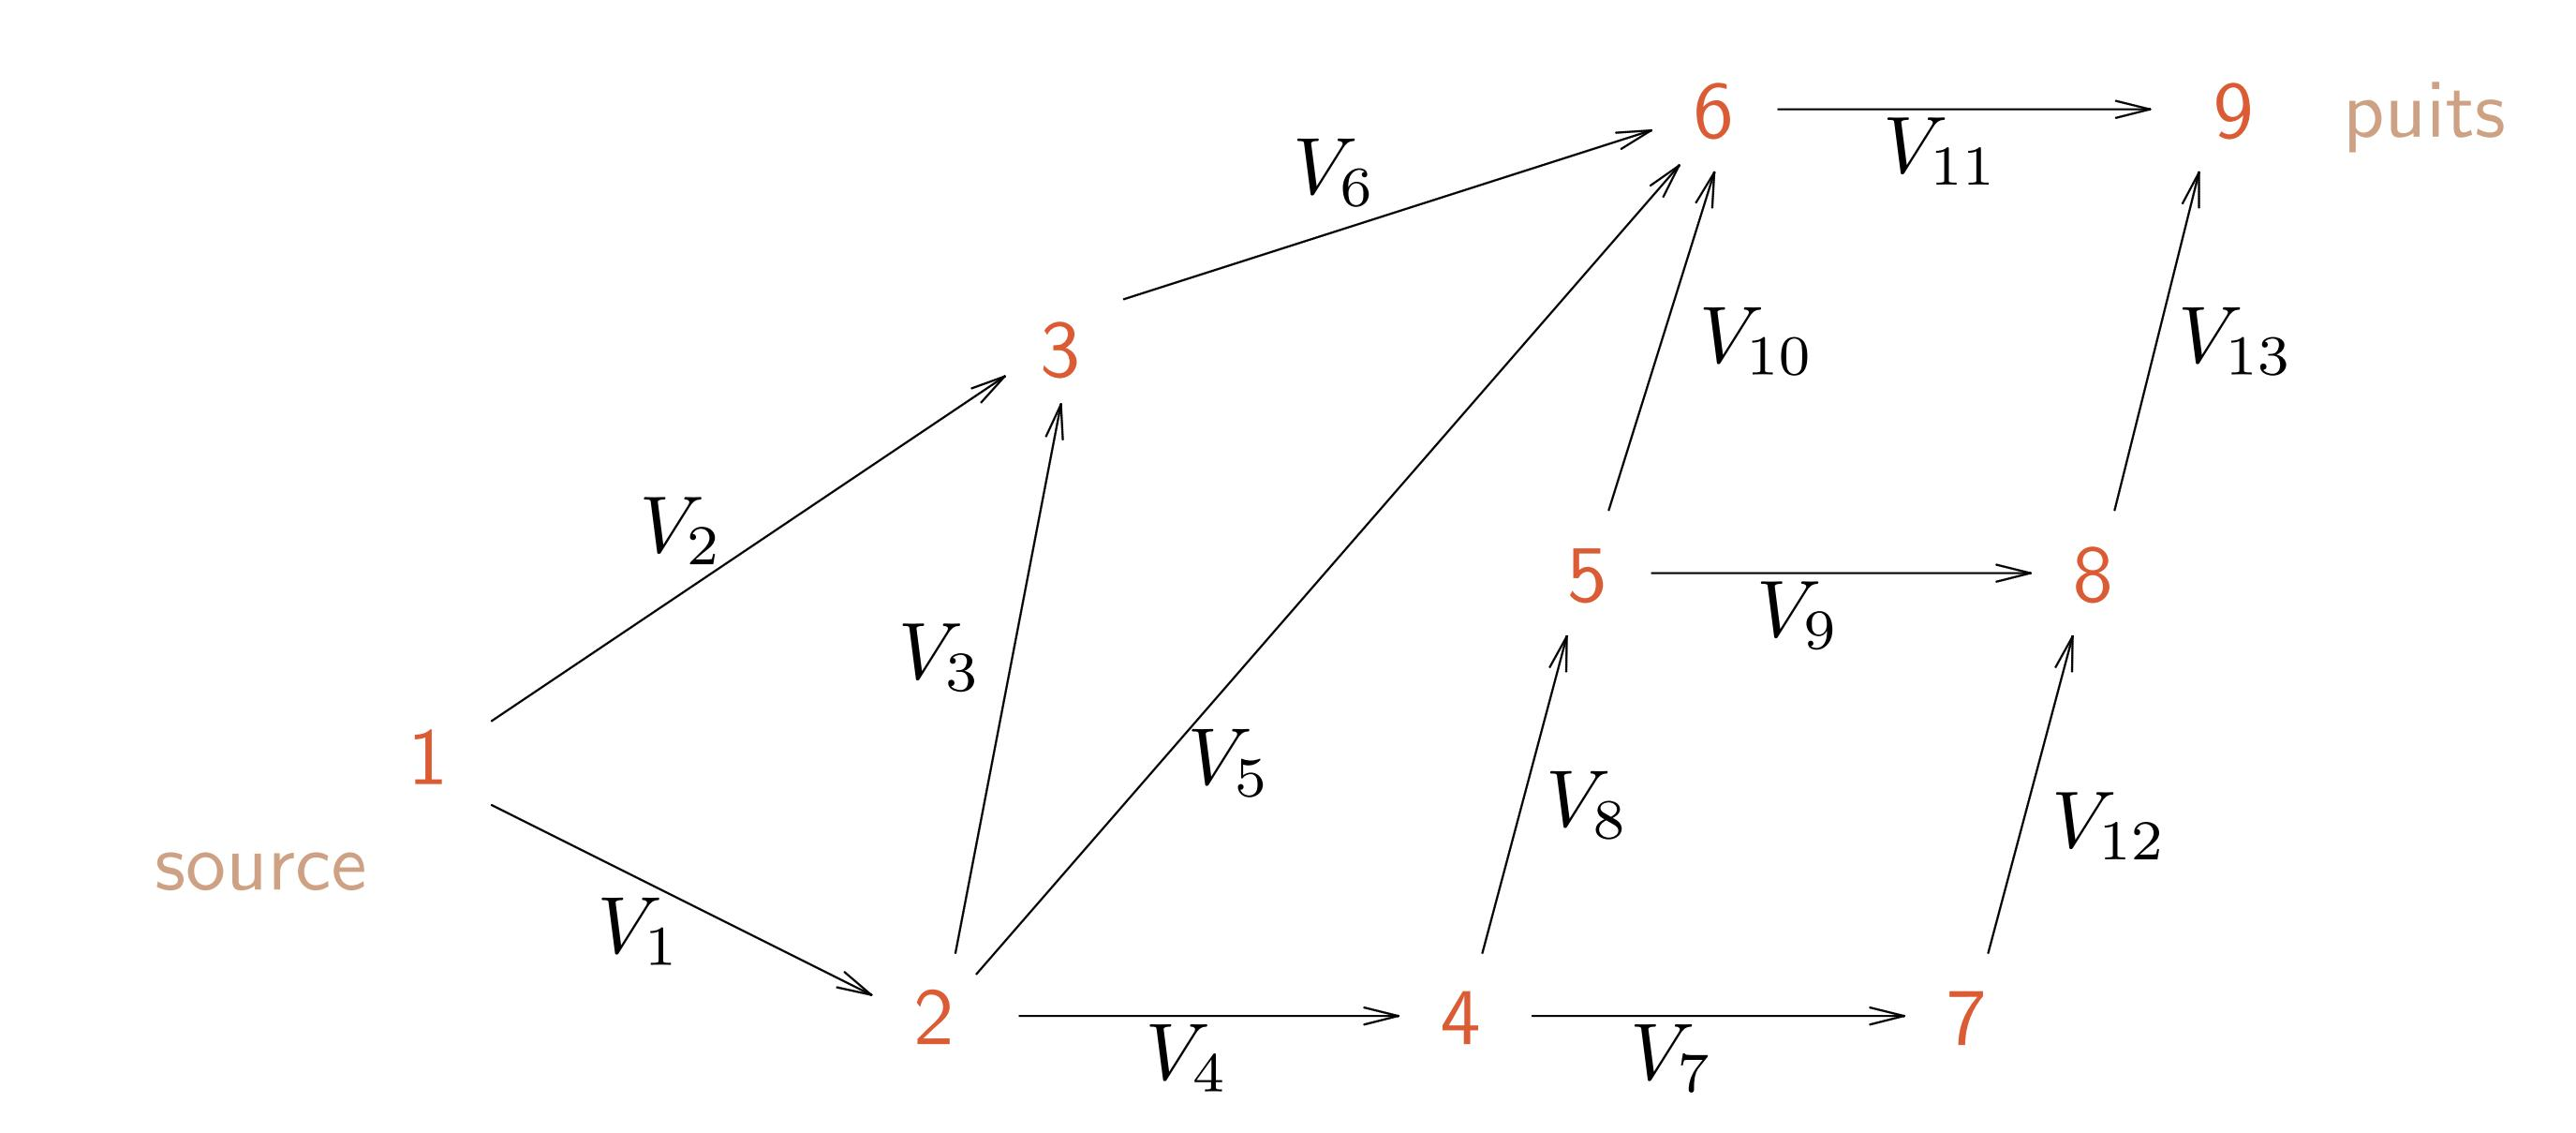
\includegraphics[scale=0.4]{san.jpg}
	\end{center}
	
\end{frame}

\begin{frame}[fragile]
\frametitle{Exemple: r\'eseau d'activit\'es stochastique}

On veut estimer $\mu = P[T > x]$, o\`u $T$ est la longueur du
plus long chemin et $x$ une constante.  

\mbox{}

On g\'en\`ere $V_j = F_j^{-1}(U_j)$ pour $X^{(1)}$ et
$V_j = F_j^{-1}(1-U_j)$ pour $X^{(2)}$.

\mbox{}

Puisque $T$ est non-d\'ecroissante en $V_j = F_j^{-1}(U_j)$, qui est
non-d\'ecroissante en $U_j$, on a un \'echantillonnage AV-concordant
et la variance est r\'eduite.

\mbox{}

En pratique, sur ce genre d'exemple, la variance est r\'eduite environ de moiti\'e.

\end{frame}

\end{document}